\section{Programación de la serie de Fourier en lenguaje C}

\subsection{Implementación de código}

\begin{enumerate} 
	\def\labelenumi{\arabic{enumi}.} 
	\item Se incluyen las bibliotecas necesarias para su funcionamiento y se define el valor de PI y las constantes necesarias, finalmente
	
	\begin{figure}[H]
		\centering
		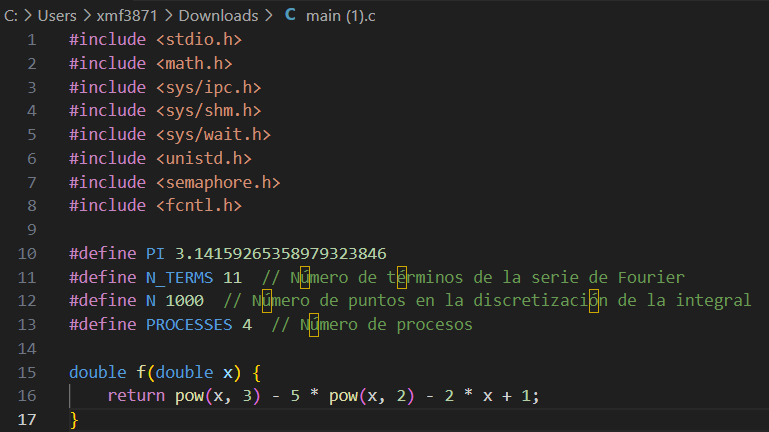
\includegraphics[width=5.55729in,height=3.12944in]{media/image18.png}
		\caption{Código}
	\end{figure}
	
	\item La función \texttt{calculate\_coefficients} se encarga de calcular los coeficientes de la serie de Fourier para un rango de términos n específico. Utiliza una técnica de sincronización con semáforos para garantizar que cada proceso realice sus cálculos de manera ordenada.
	
	\begin{figure}[H]
		\centering
		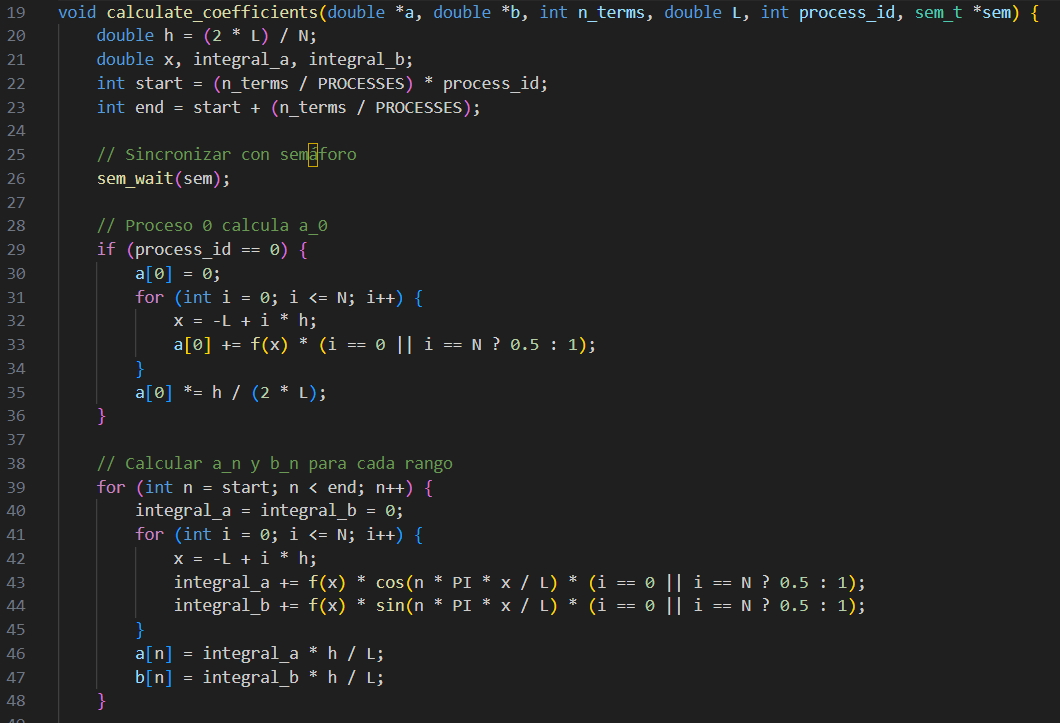
\includegraphics[width=5.64741in,height=3.85562in]{media/image39.png}
		\caption{Función \texttt{calculate\_coefficients}}
	\end{figure}
	
	\item La función \texttt{fourier\_approximation} calcula la aproximación de la función original utilizando los coeficientes de la serie de Fourier.
	
	\begin{figure}[H]
		\centering
		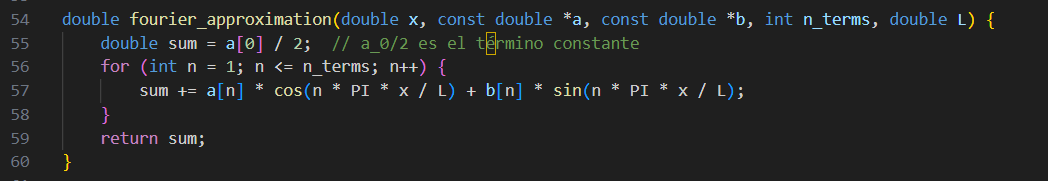
\includegraphics[width=6.26772in,height=1.08333in]{media/image11.png}
		\caption{Función \texttt{fourier\_approximation}}
	\end{figure}
	
	\item La función \texttt{export\_to\_csv} exporta los resultados a un archivo CSV que contiene los valores de x, la función original y la aproximación de la serie de Fourier y\_fourier.
	
	\begin{figure}[H]
		\centering
		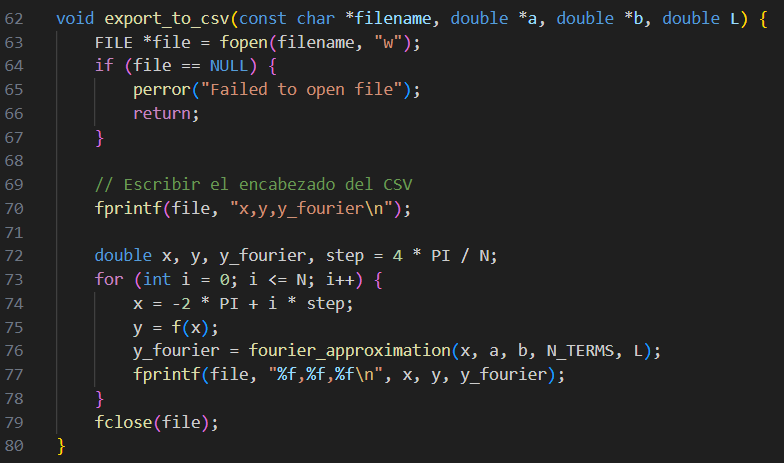
\includegraphics[width=5.02604in,height=2.61756in]{media/image50.png}
		\caption{Función \texttt{export\_to\_csv}}
	\end{figure}
	
	\item En la función \texttt{main}, se crea un segmento de memoria compartida para almacenar los coeficientes a y b, se crea un semáforo para la sincronización entre procesos y se generan varios procesos hijos para calcular los coeficientes de la serie de Fourier en paralelo. Después de que todos los procesos hayan terminado de calcular los coeficientes, se exportan los resultados a un archivo CSV y se liberan los recursos utilizados.
	
	\begin{figure}[H]
		\centering
		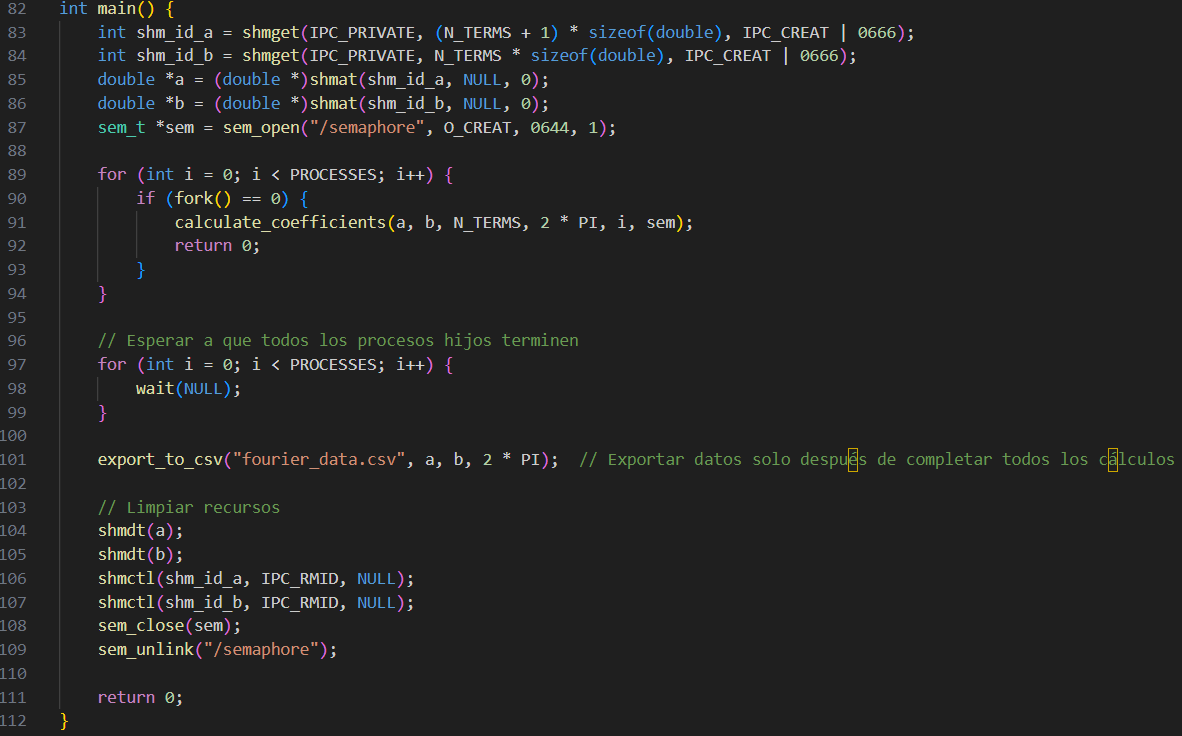
\includegraphics[width=6.26772in,height=3.90278in]{media/image7.png}
		\caption{Función \texttt{main}}
	\end{figure}
	
\end{enumerate}

\subsection{Ejecución del código}

\begin{enumerate} 
	\def\labelenumi{\arabic{enumi}.} 
	\item Ejecución de código en GNU/Linux
	
	\begin{figure}[H]
		\centering
		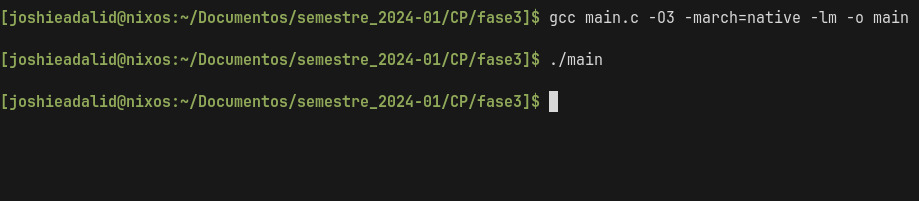
\includegraphics[width=6.26772in,height=1.375in]{media/image29.png}
		\caption{Ejecución en GNU/Linux}
	\end{figure}
	
	\item Visualización del archivo generado. Para cada x, su evaluación en la función a aproximar, y su aproximación de la serie de Fourier.
	
	\begin{figure}[H]
		\centering
		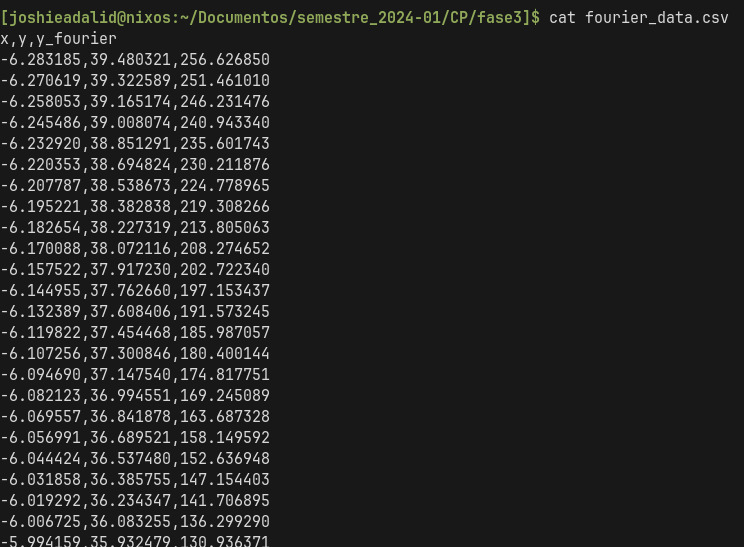
\includegraphics[width=5.16146in,height=3.79822in]{media/image37.png}
		\caption{Aproximación para la serie de Fourier}
	\end{figure}
	
	\begin{figure}[H]
		\centering
		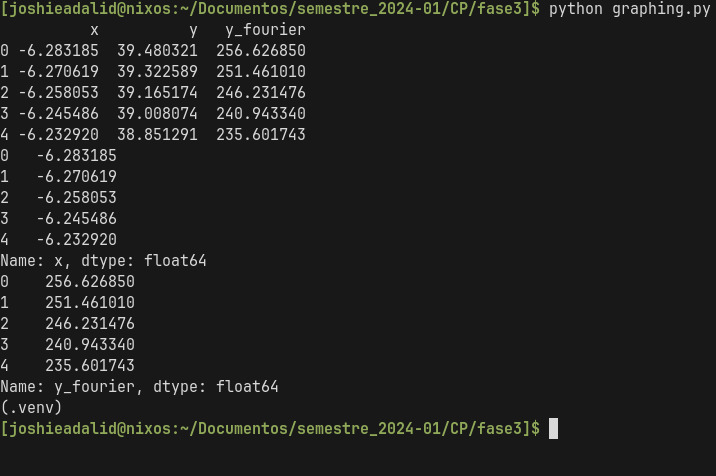
\includegraphics[width=5.16146in,height=3.42309in]{media/image25.png}
		\caption{Aproximación para la serie de Fourier}
	\end{figure}
	
	\item Gráfica generada
	
	\begin{figure}[H]
		\centering
		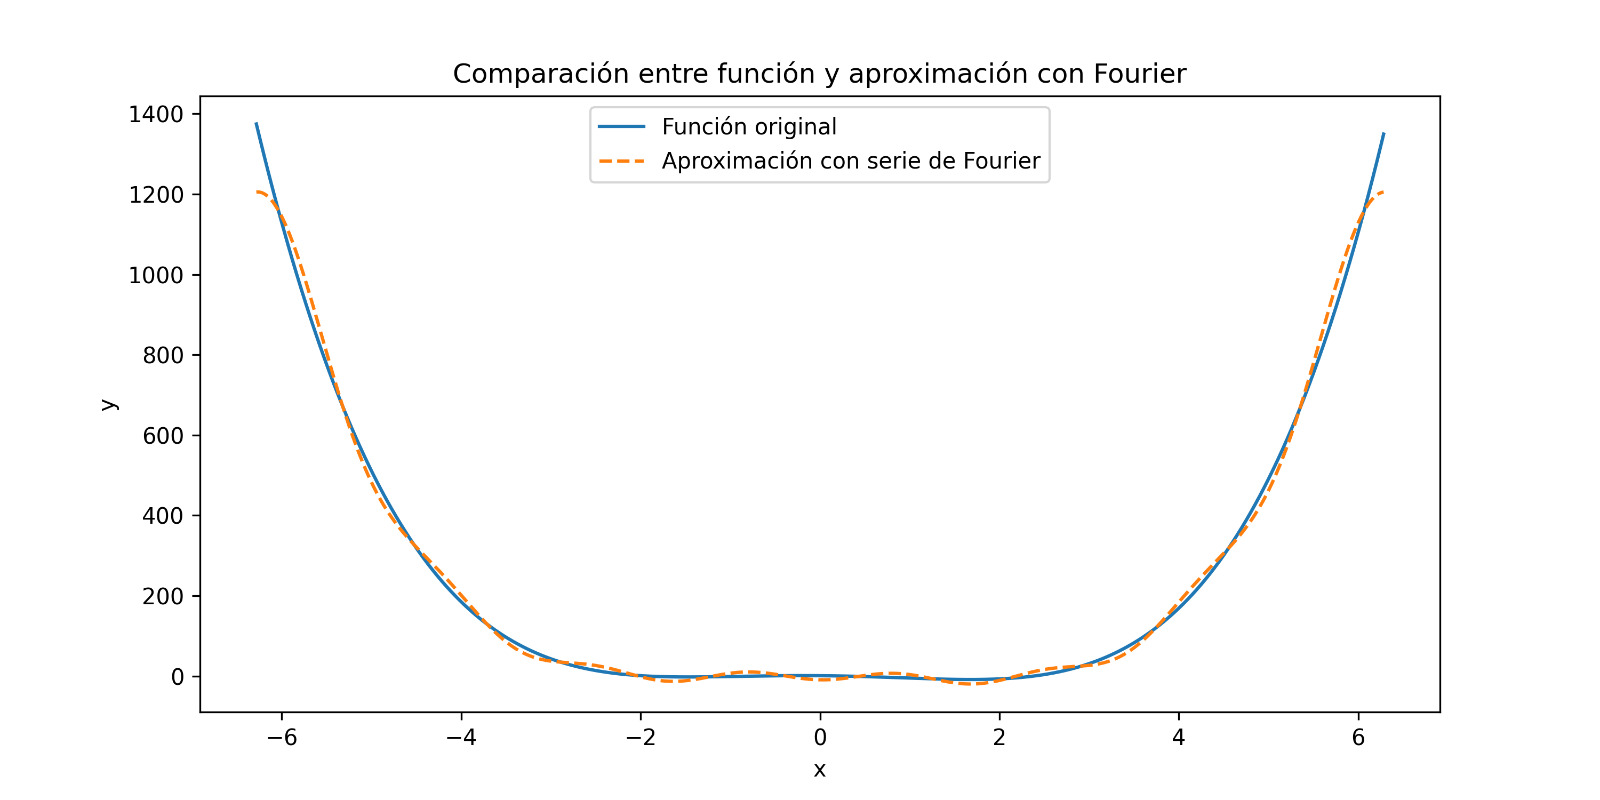
\includegraphics[width=6.26772in,height=3.13889in]{media/image12.png}
		\caption{Gráfica original y aproximación de Fourier en C}
	\end{figure}
	
\end{enumerate}

\subsection{Implementación de código con hilos}

En este apartado se mostrará y explicará el código implementado ahora con hilos en lugar de memoria compartida y semáforos.

\begin{enumerate} 
	\def\labelenumi{\arabic{enumi}.} 
	\item En primer lugar, se incluyen las bibliotecas necesarias para utilizar las funciones básicas y las funciones de hilos como se muestran en la imagen 13, así como definir unas constantes que nos ayudarán a ejecutar el programa con hilos.
	
	\begin{figure}[H]
		\centering
		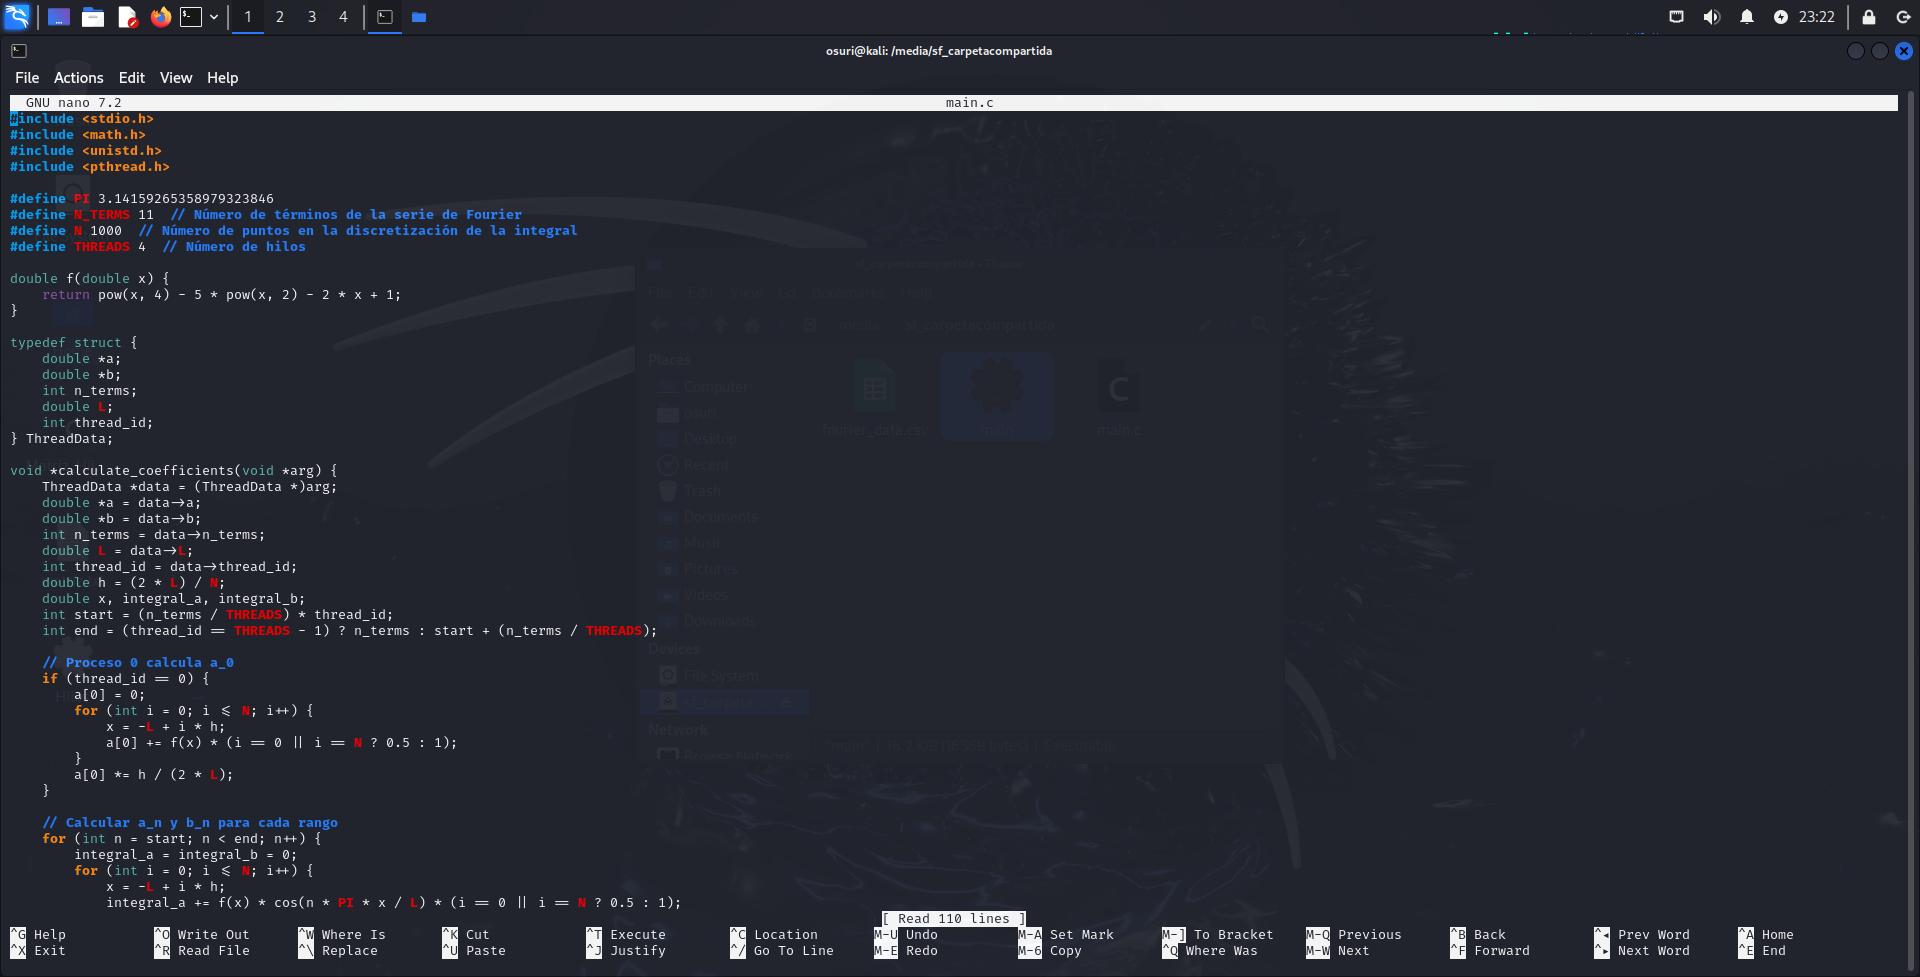
\includegraphics[width=4.53385in,height=1.24967in]{media/image4.png}
		\caption{Código 1. Fuente: Autoría propia}
	\end{figure}
	
	\item En la imagen 14 se define la estructura básica de la serie original y se crea la estructura de un hilo para que tenga los datos de la ecuación de la serie, así como los valores que debe de calcular, para almacenar múltiples tipos de datos y no entre en conflicto.
	
	\begin{figure}[H]
		\centering
		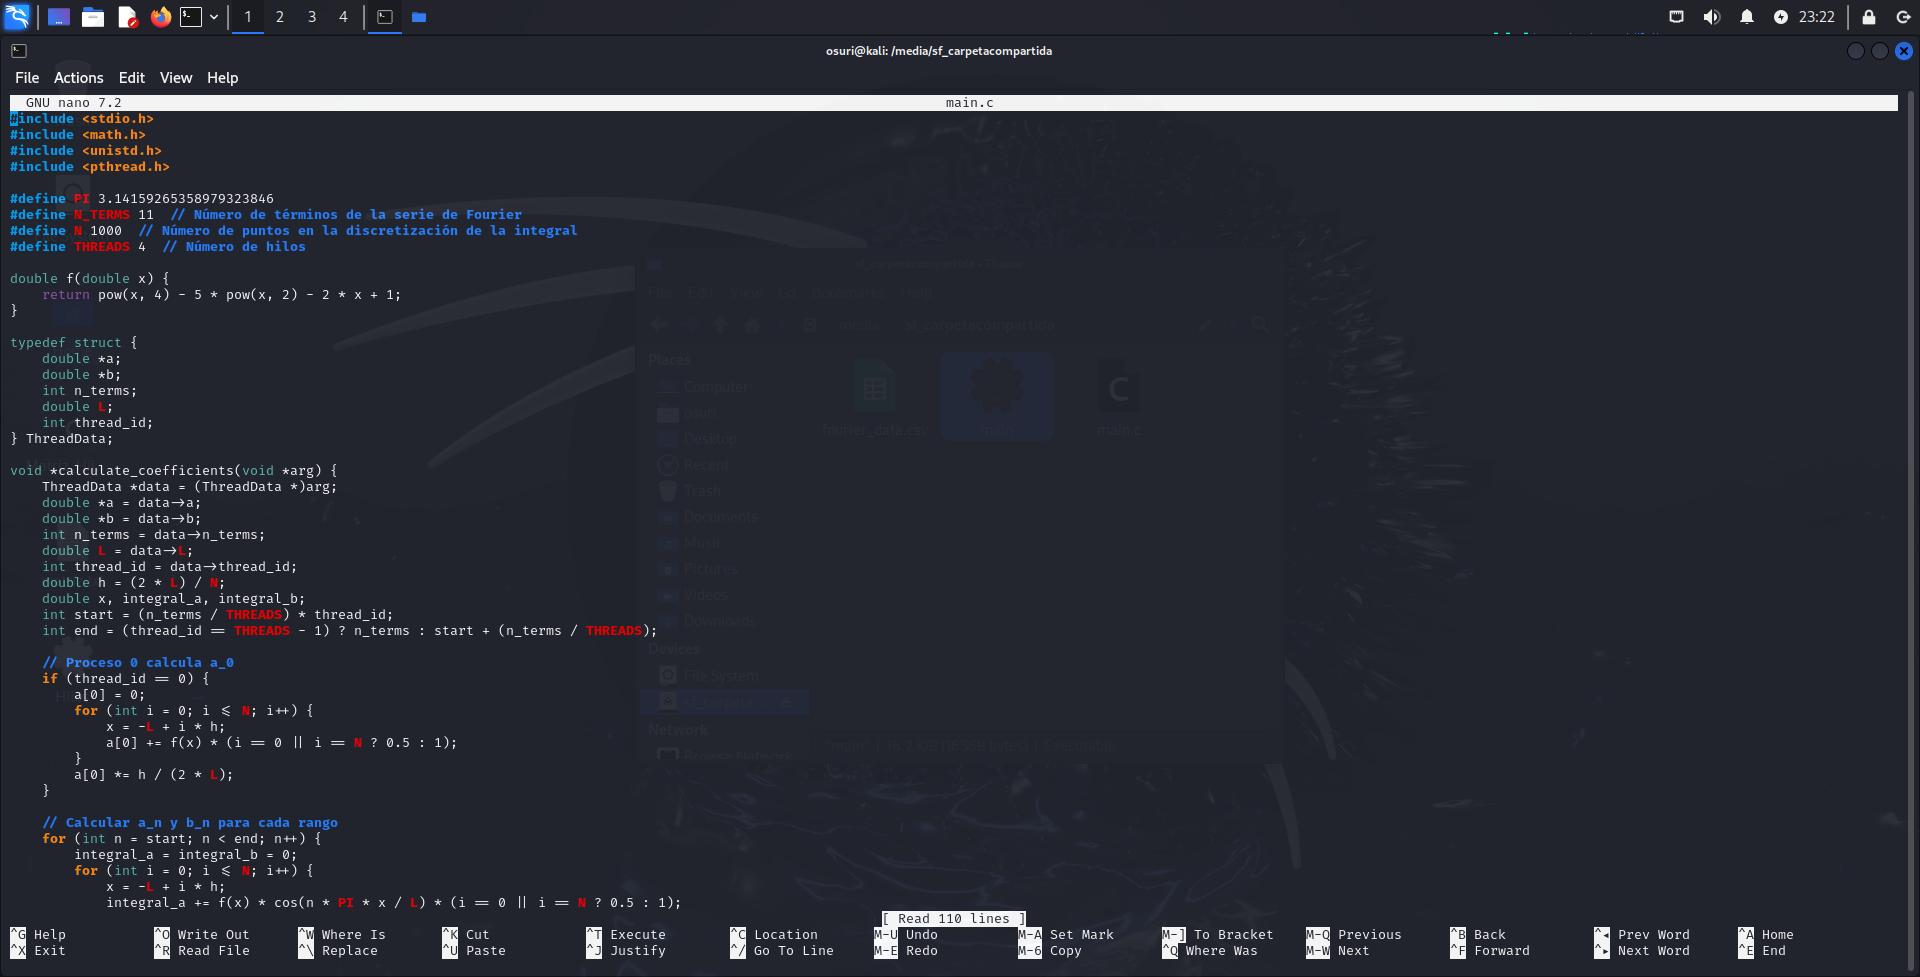
\includegraphics[width=3.15in,height=1.54172in]{media/image4.png}
		\caption{Código 2. Fuente: Autoría propia}
	\end{figure}
	
	\item En la imagen 15, se define una función para resolver la serie de Fourier por medio de hilos, se divide la información para que pueda ser ejecutada miles de veces, y se crean los hilos separados para resolver los cálculos. Se pone separado el cálculo de \(a0\) porque sólo se calcula una vez, mientras que an y bn deben ser calculados tantas veces como \(n\) existan.
	
	\begin{figure}[H]
		\centering
		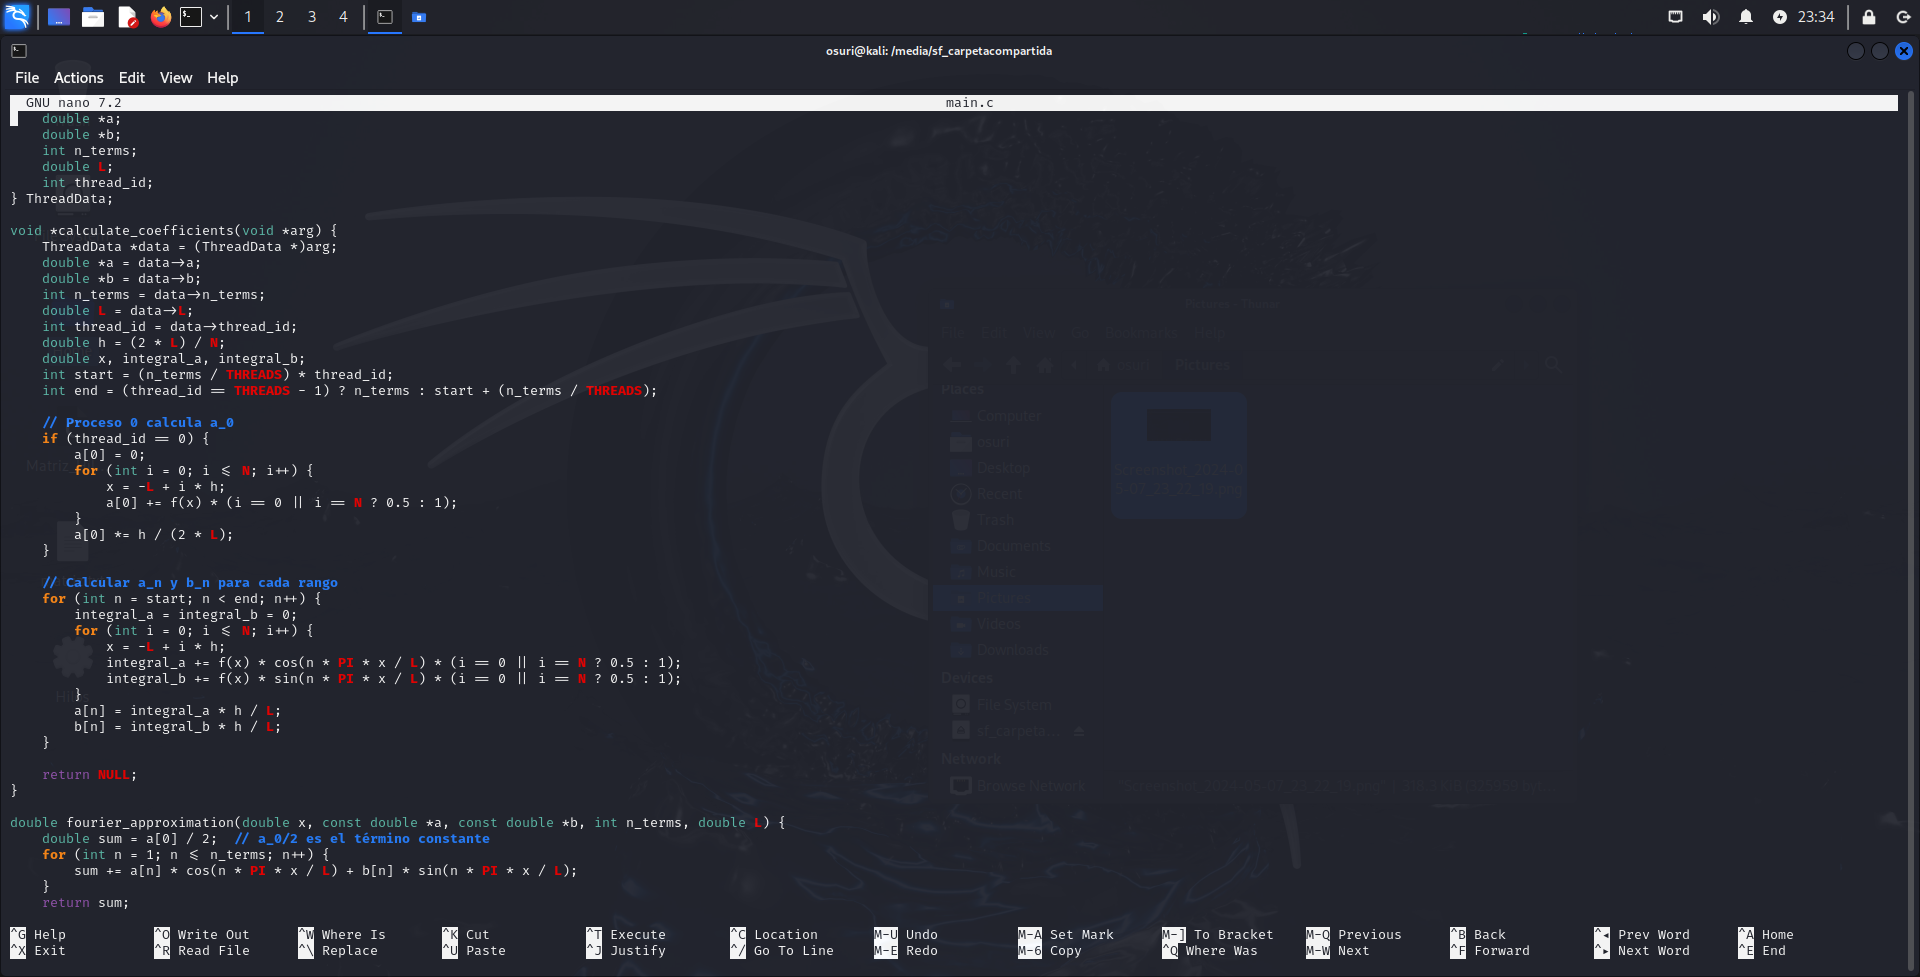
\includegraphics[width=3.00416in,height=2.52623in]{media/image17.png}
		\caption{Código 3. Fuente: Autoría propia}
	\end{figure}
	
	\item En la imagen 16 se crea una función de aproximación con la serie original para comparar los valores.
	
	\begin{figure}[H]
		\centering
		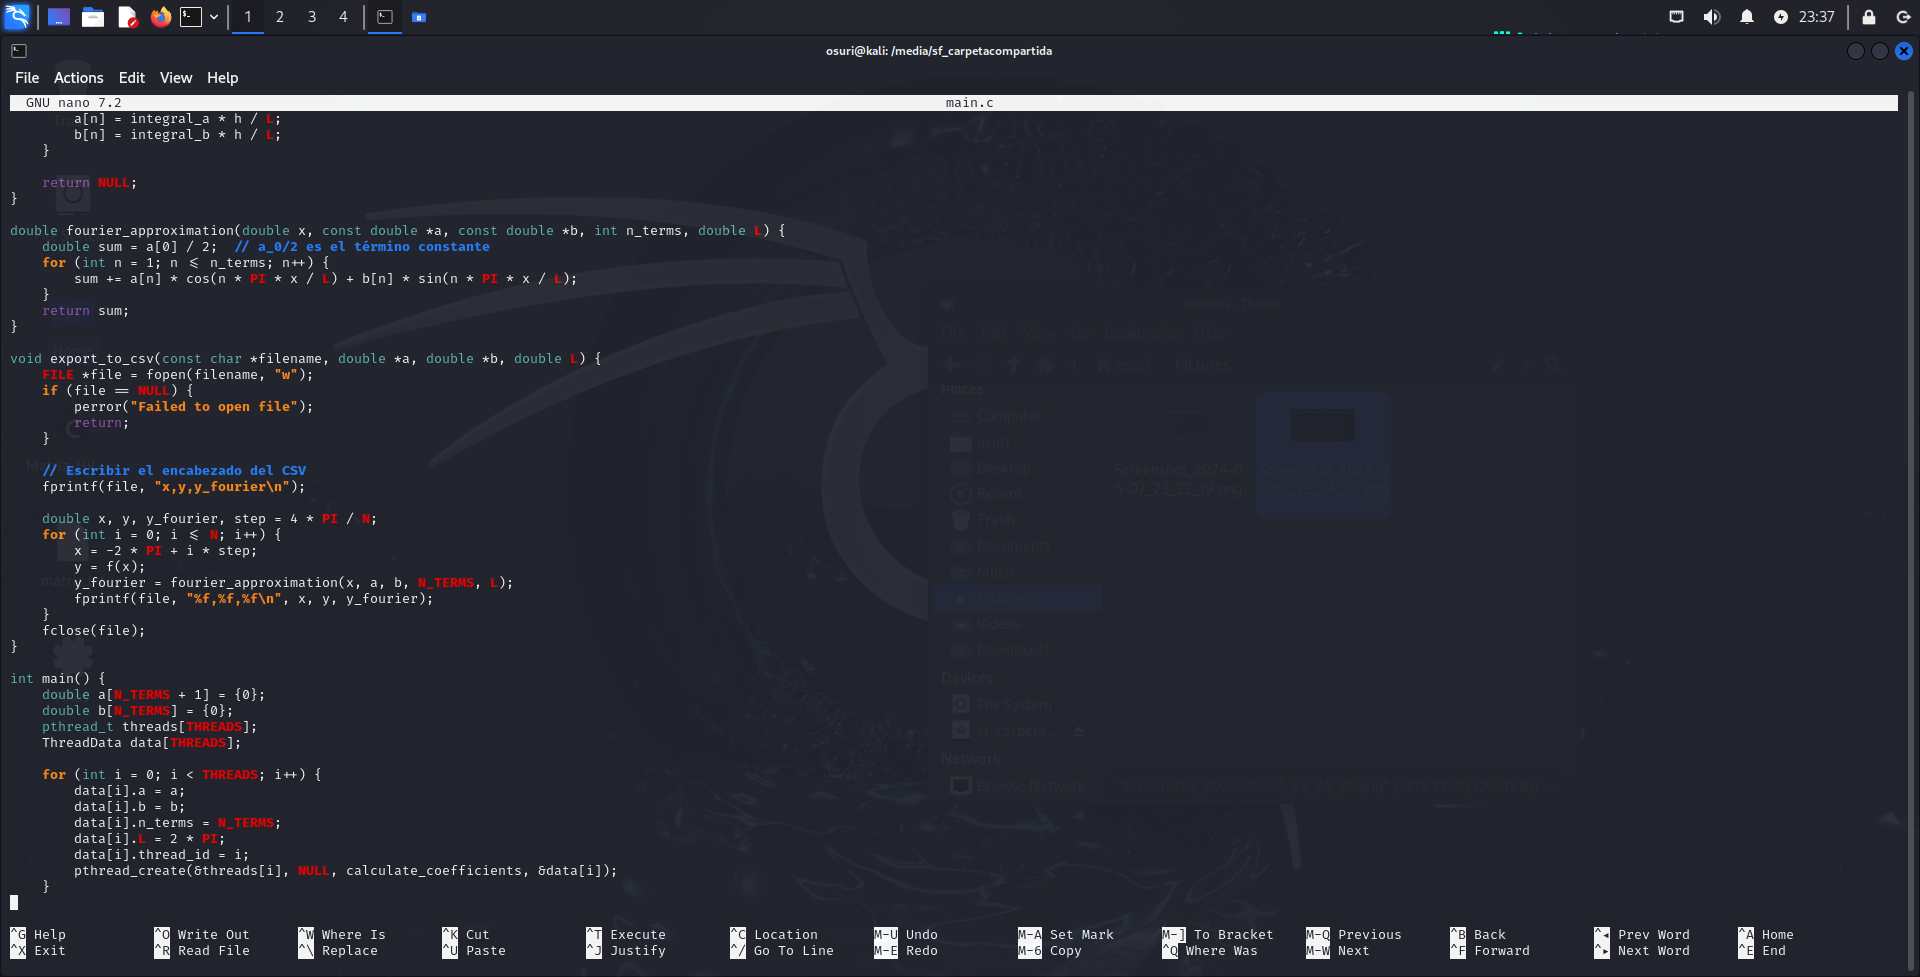
\includegraphics[width=4.31145in,height=0.71292in]{media/image27.png}
		\caption{Código 4. Fuente: Autoría propia}
	\end{figure}
	
	\item En la imagen 17, se crea la función para exportar los cálculos exitosos a un archivo CSV para poder guardarlos y consultarlos.
	
	\begin{figure}[H]
		\centering
		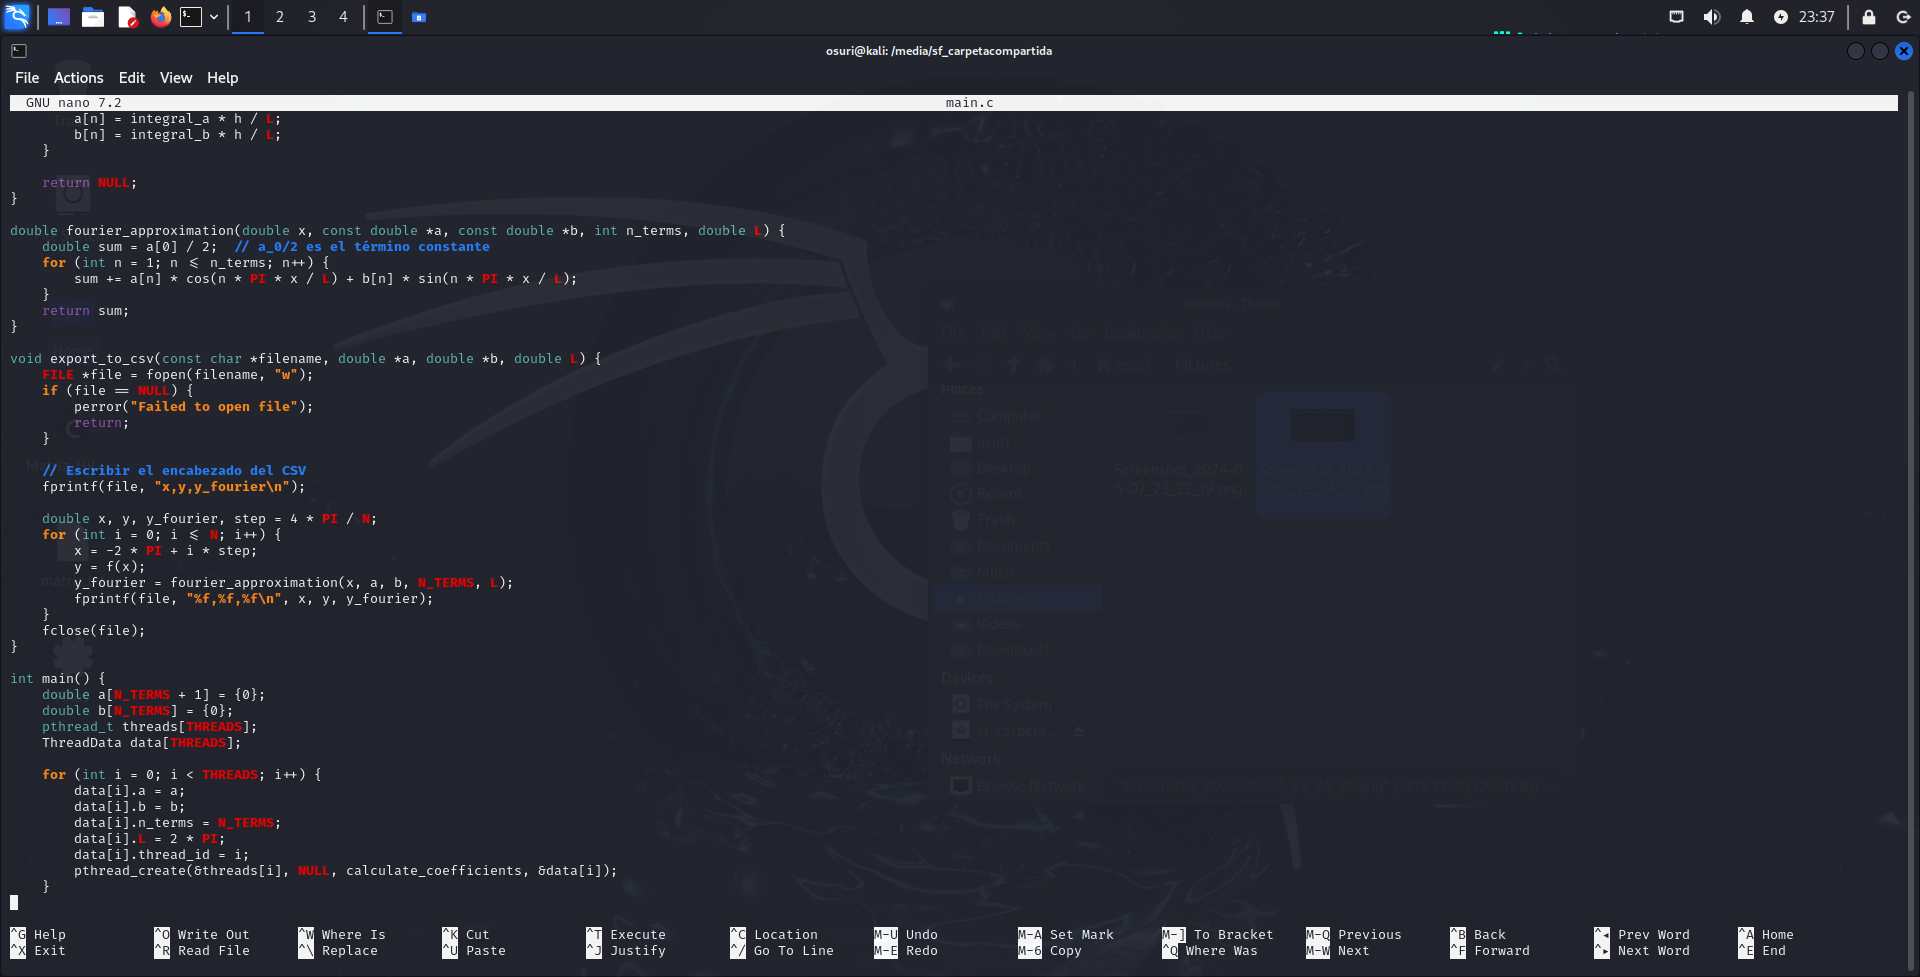
\includegraphics[width=4.19531in,height=2.2036in]{media/image27.png}
		\caption{Código 5. Fuente: Autoría propia}
	\end{figure}
	
	\item En la imagen 18, se puede observar el programa main, donde se ejecuta el proceso principal, se crean los hilos de acuerdo a la cantidad de veces que se ejecutará la secuencia, en este caso 1000, se utilizará la estructura del hilo definida con anterioridad para ejecutar los hilos, y finalmente se utilizará la función para exportar a CSV para guardar los datos.
	
	\begin{figure}[H]
		\centering
		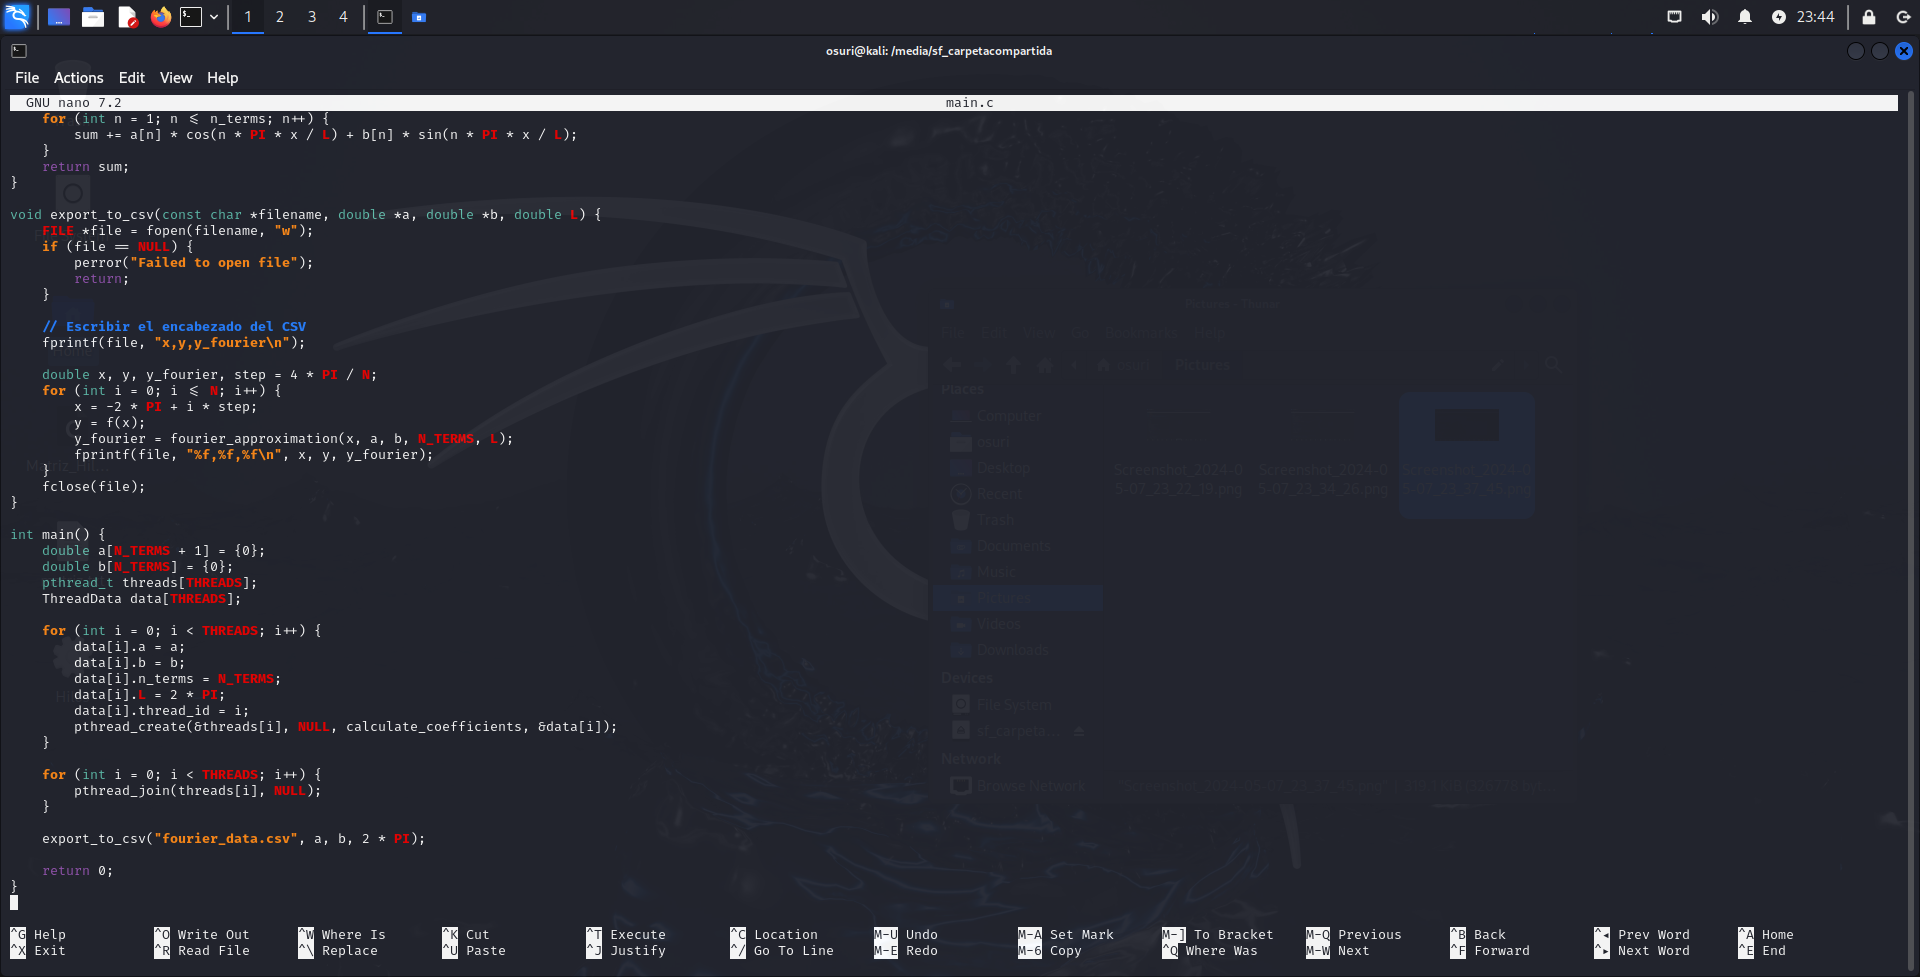
\includegraphics[width=3.82031in,height=2.4068in]{media/image5.png}
		\caption{Código 6. Fuente: Autoría propia}
	\end{figure}
	
\end{enumerate}

\subsection{Ejecución del código con hilos}

\begin{enumerate} 
	\def\labelenumi{\arabic{enumi}.} 
	\item Compilación y ejecución (ver imagen 19).
	
	\begin{figure}[H]
		\centering
		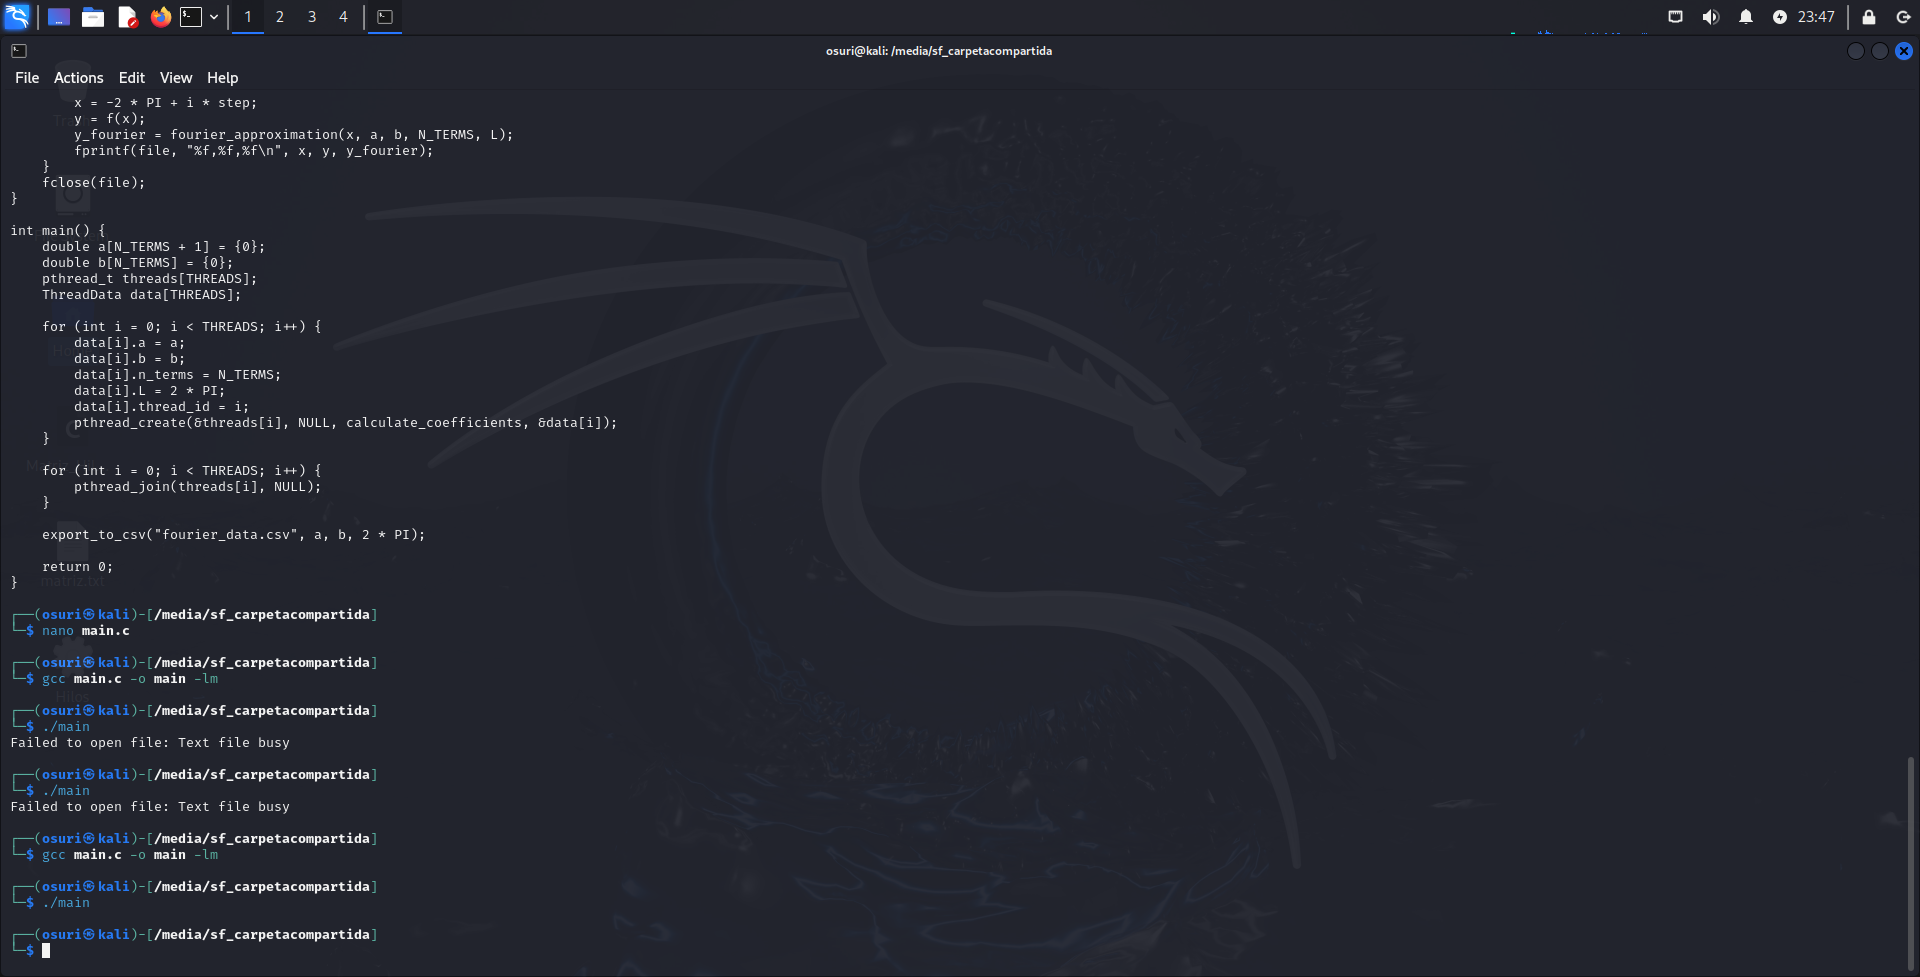
\includegraphics[width=3.46875in,height=0.8384in]{media/image36.png}
		\caption{Compilación y ejecución. Fuente: Autoría propia}
	\end{figure}
	
	\item Visualización menor de datos, solo se utilizan ciertos datos para no saturar el documento (ver imagen 20).
	
	\begin{figure}[H]
		\centering
		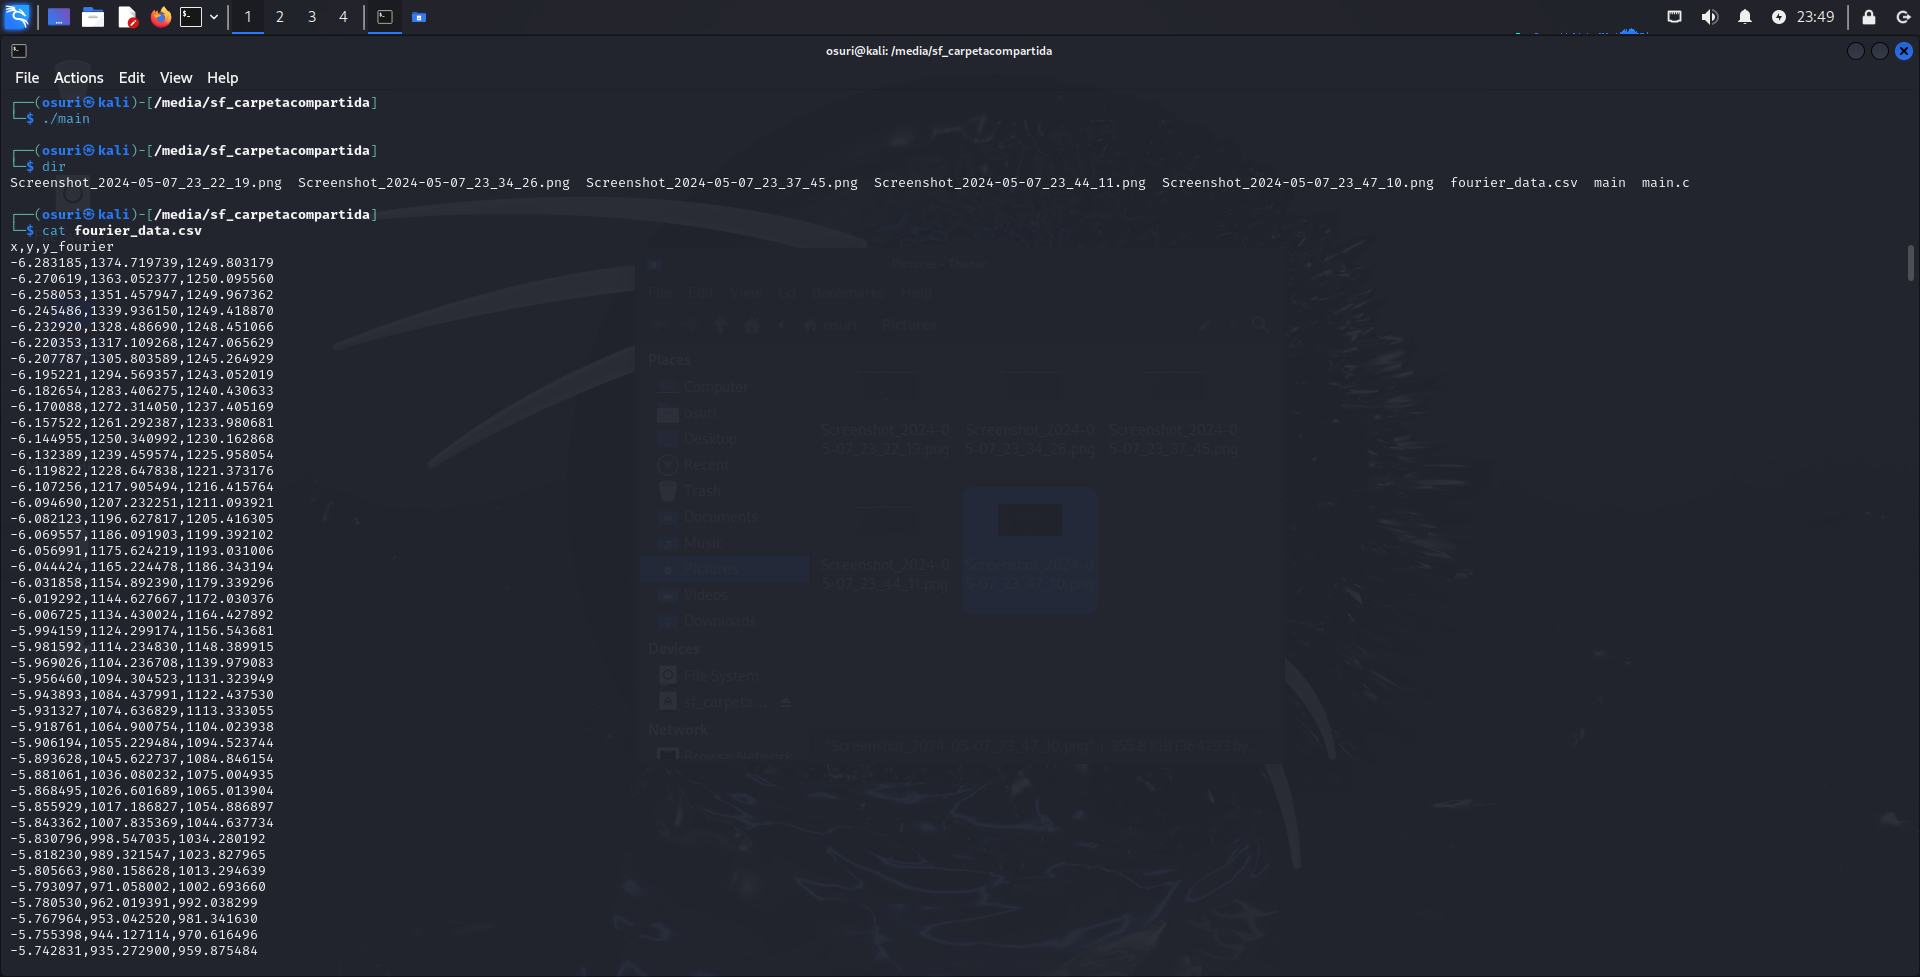
\includegraphics[width=2.29583in,height=4.29598in]{media/image35.png}
		\caption{Datos de archivo CSV. Fuente: Autoría propia}
	\end{figure}
	
	\item Gráfica generada por este conjunto de datos (ver figura 5)
	
	\begin{figure}[H]
		\centering
		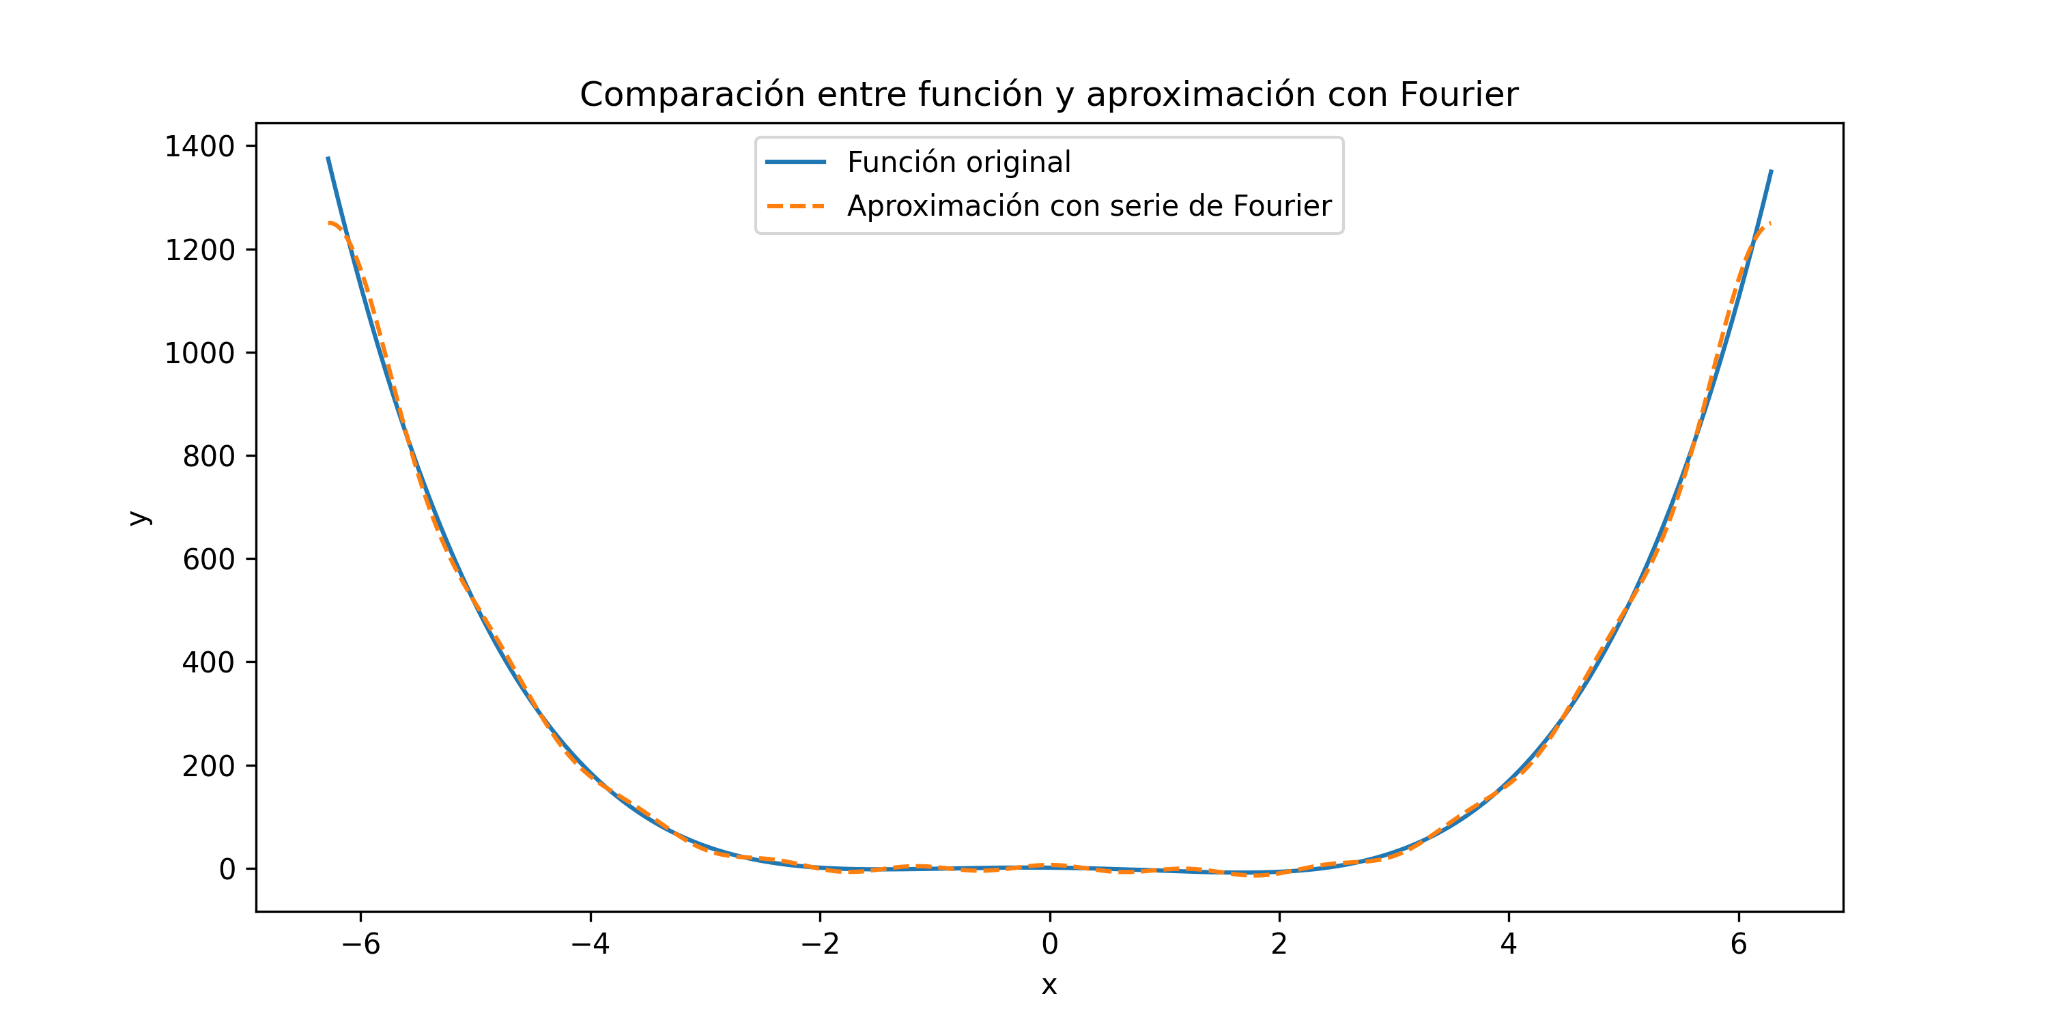
\includegraphics[width=6.26772in,height=3.13889in]{media/image30.png}
		\caption{Gráfica generada. Fuente: Autoría propia}
	\end{figure}
	
\end{enumerate}

\subsection{Ejecución del código con MPI}
\begin{figure}[H]
	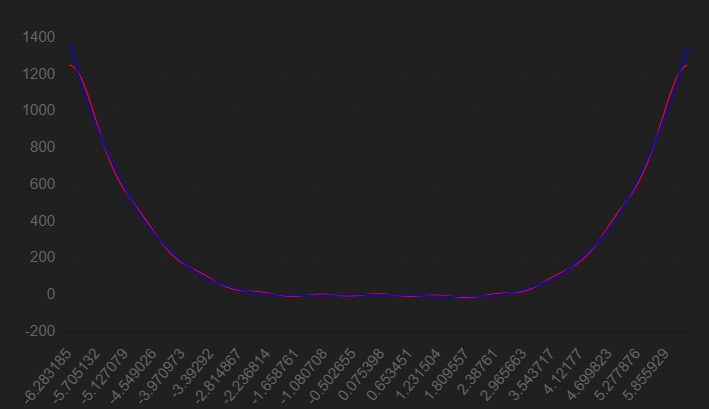
\includegraphics[width=0.8\textwidth]{media/mpi_grafica.jpeg}
	\caption{Comparación de la función original contra la aproximación de la serie de Fourier, calculado con la tecnología de MPI}
\end{figure}

\begin{figure}[H]
	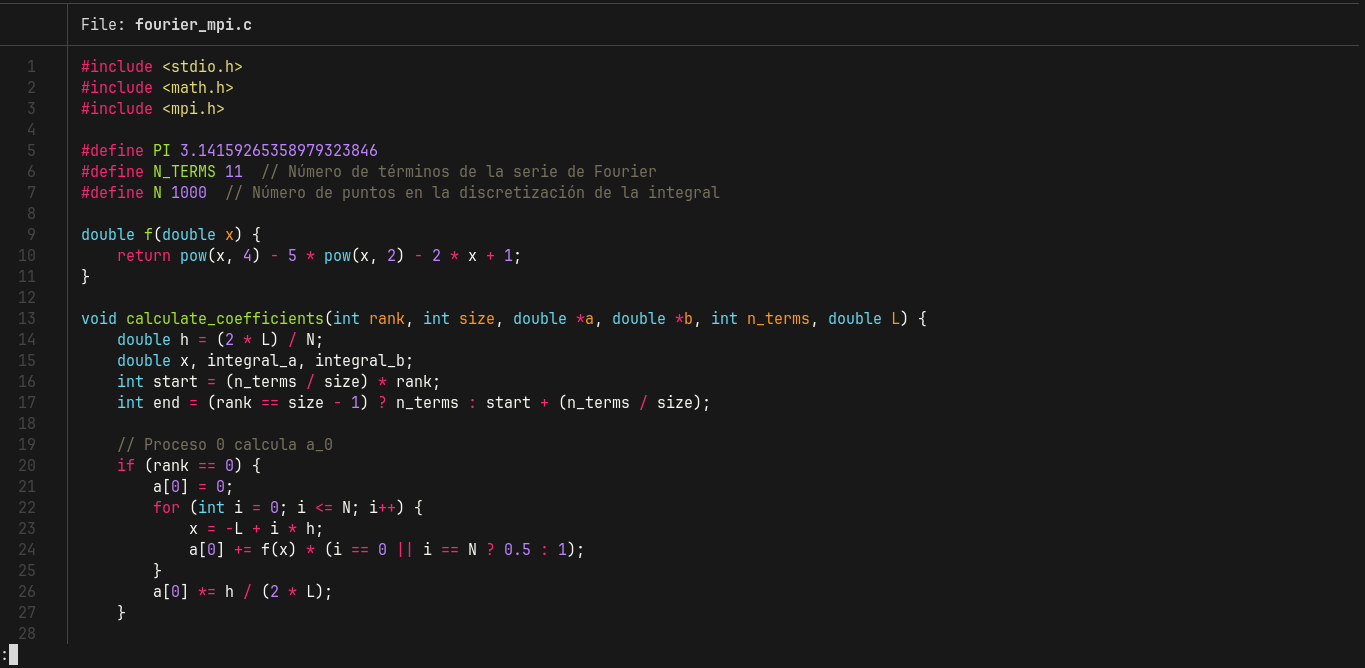
\includegraphics[width=0.8\textwidth]{media/mpi_codigo_1.png}
	\caption{Fragmento del código fuente en C para MPI. Parte 1 de 4.}
\end{figure}
\begin{figure}[H]
	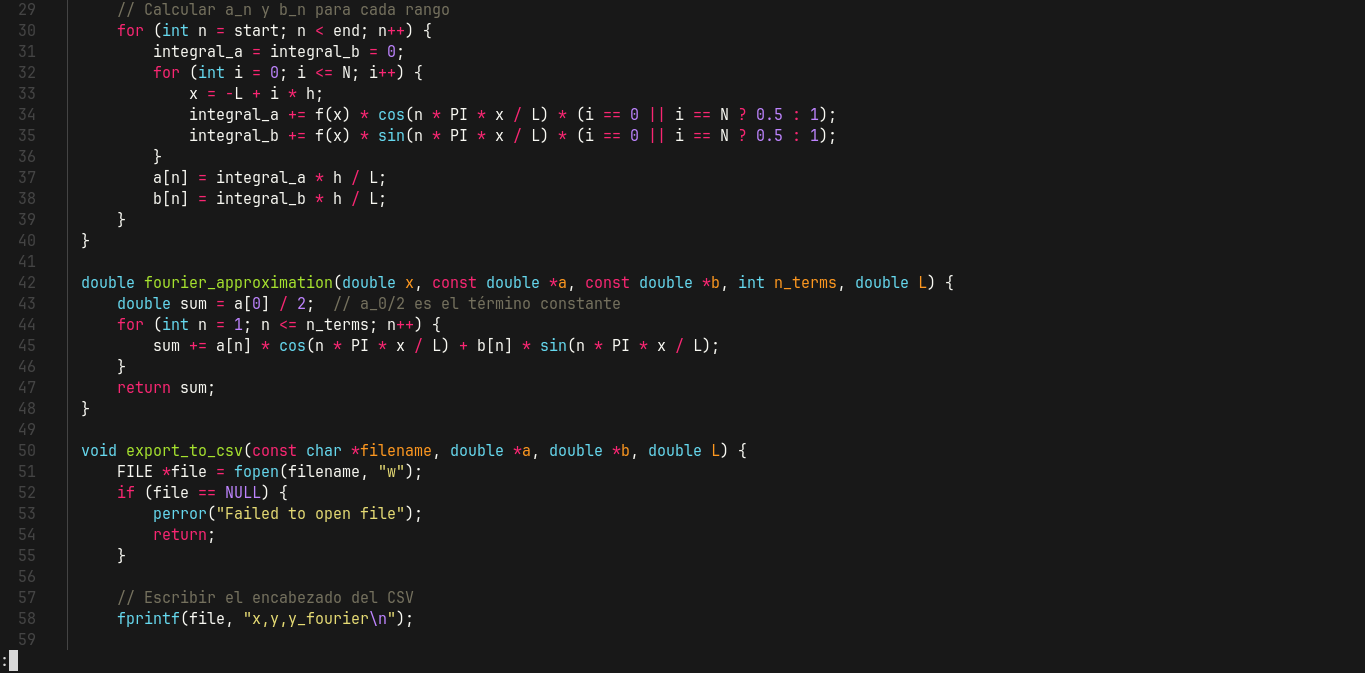
\includegraphics[width=0.8\textwidth]{media/mpi_codigo_2.png}
	\caption{Fragmento del código fuente en C para MPI. Parte 2 de 4.}
\end{figure}
\begin{figure}[H]
	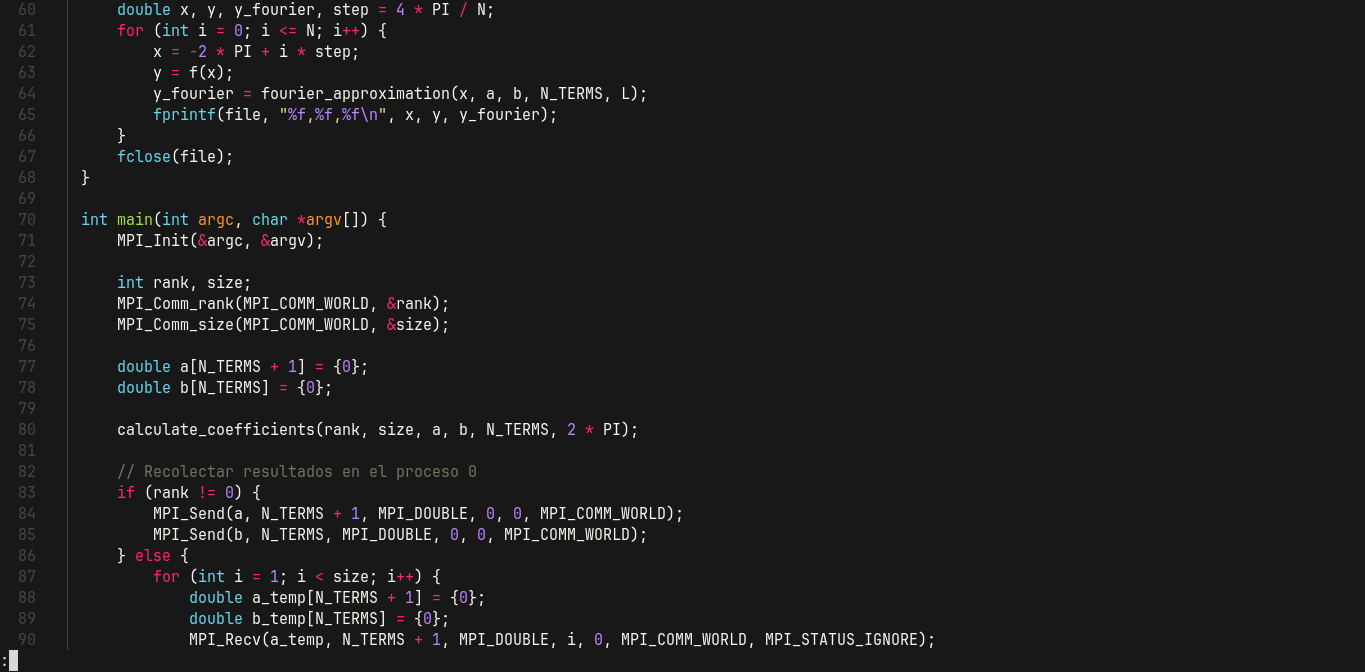
\includegraphics[width=0.8\textwidth]{media/mpi_codigo_3.png}
	\caption{Fragmento del código fuente en C para MPI. Parte 3 de 4.}
\end{figure}
\begin{figure}[H]
	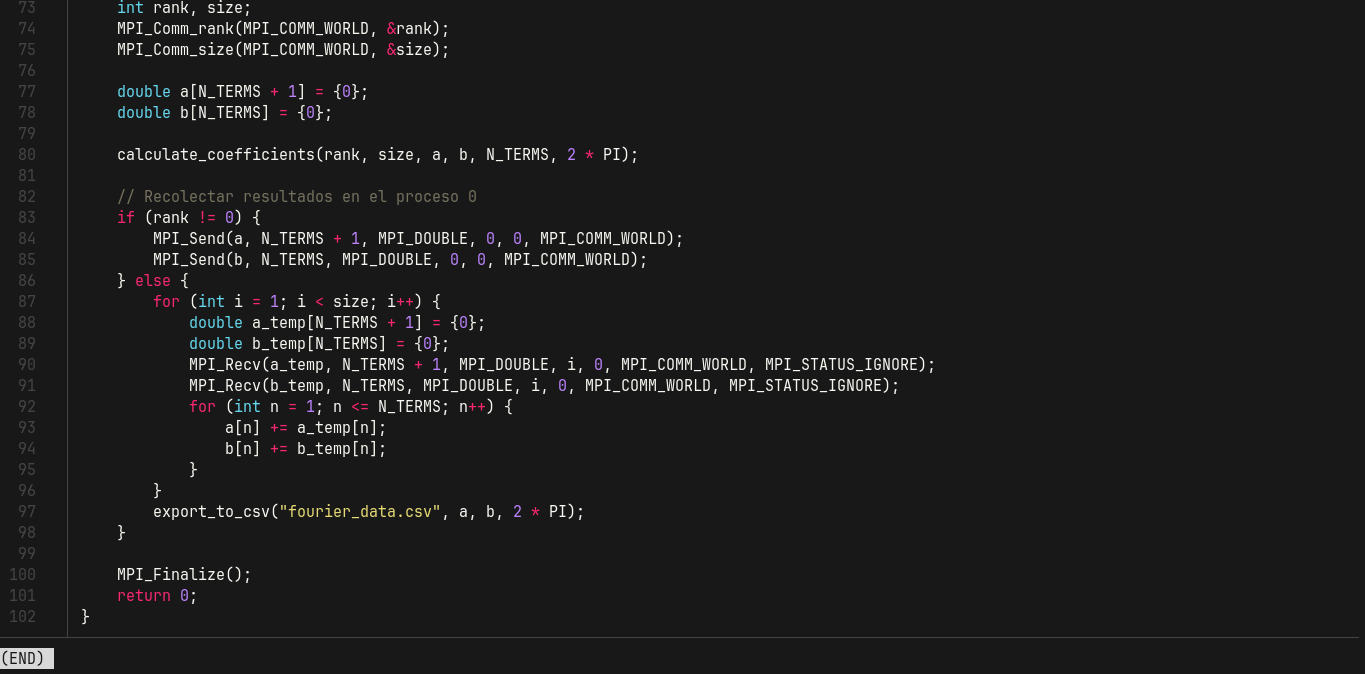
\includegraphics[width=0.8\textwidth]{media/mpi_codigo_4.png}
	\caption{Fragmento del código fuente en C para MPI. Parte 4 de 4.}
\end{figure}

\subsection{Ejecución del código con CUDA}
\begin{figure}[H]
	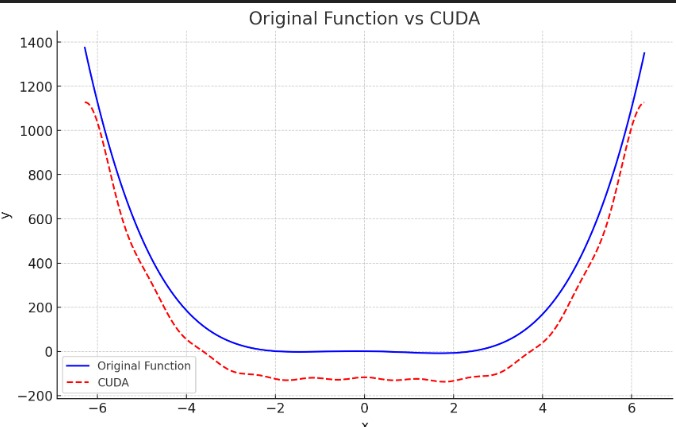
\includegraphics[width=0.8\textwidth]{media/resultados_cuda.jpeg}
	\caption{Comparación entre la función original y su implementación en CUDA. La gráfica muestra cómo la función original (línea azul continua) y la versión paralelizada con CUDA (línea roja discontinua) se comportan de manera diferente en términos de rendimiento y precisión. Se observa una discrepancia notable en los valores de la función, especialmente en los extremos.}
	\label{fig:comparacion_cuda}
\end{figure}

\begin{figure}
	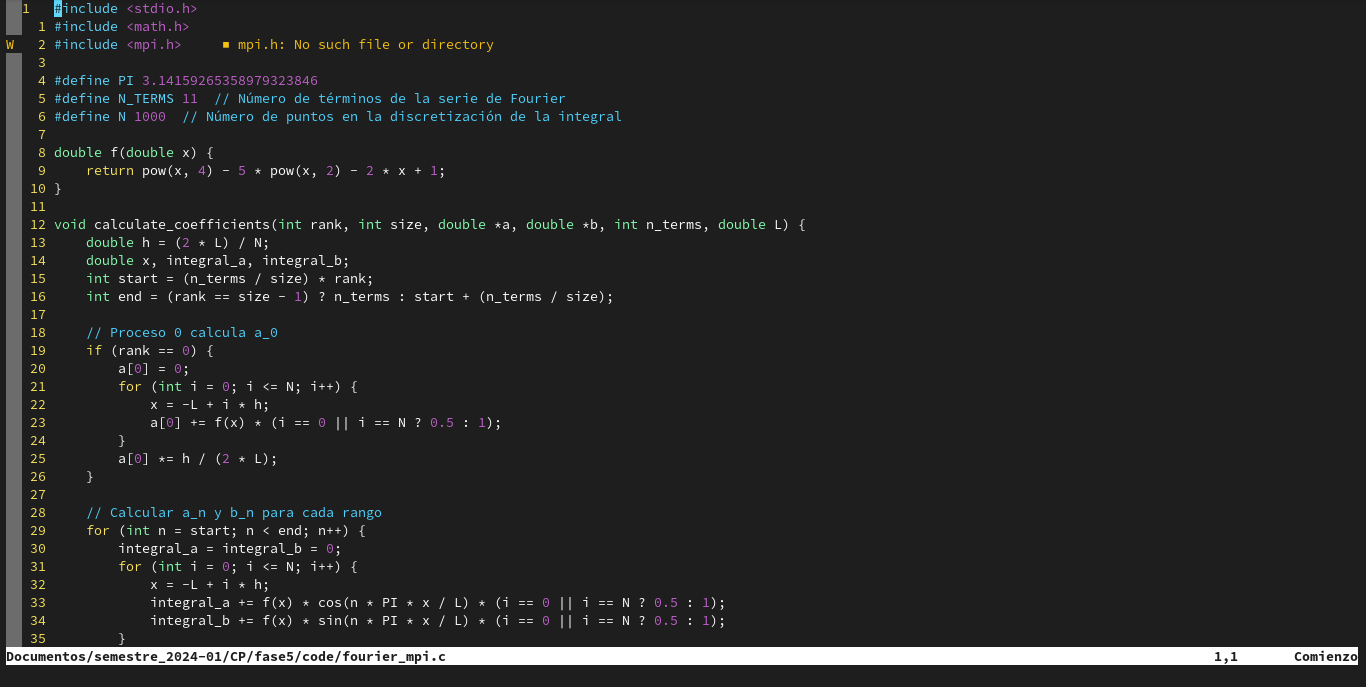
\includegraphics[width=\textwidth]{media/codigo_cuda_1.png}
	\caption{Fragmento del código fuente en C para CUDA. Imagen 1 de 4.}
	\label{img:codigo_cuda_1}
\end{figure}

\begin{figure}
	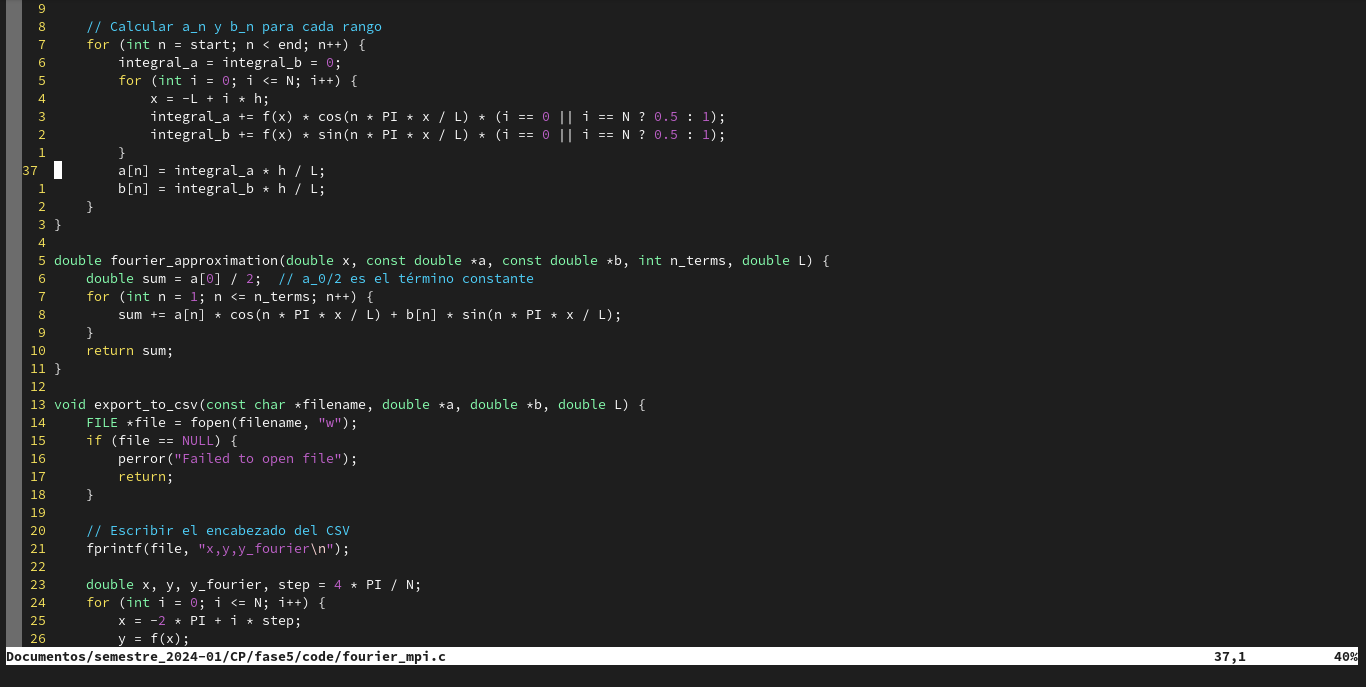
\includegraphics[width=\textwidth]{media/codigo_cuda_2.png}
	\caption{Fragmento del código fuente en C para CUDA. Imagen 2 de 4.}
	\label{img:codigo_cuda_2}
\end{figure}
\begin{figure}
	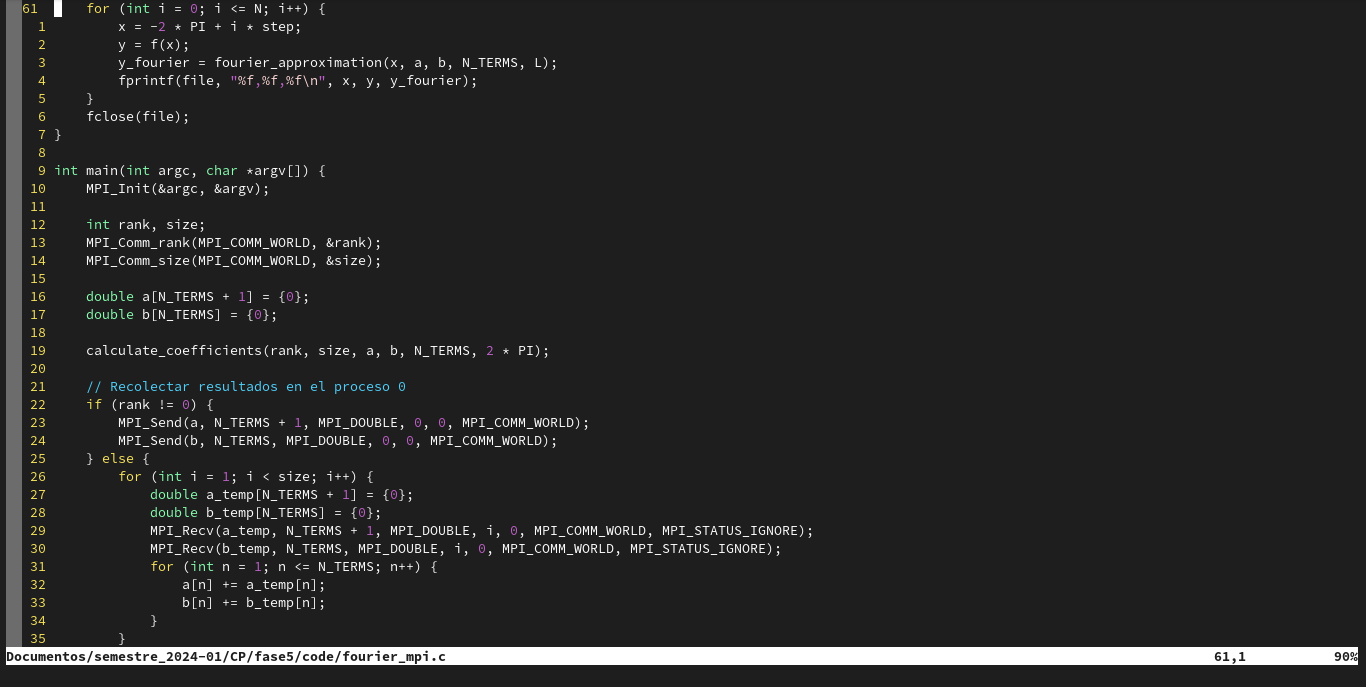
\includegraphics[width=\textwidth]{media/codigo_cuda_3.png}
	\caption{Fragmento del código fuente en C para CUDA. Imagen 3 de 4.}
	\label{img:codigo_cuda_3}
\end{figure}
\begin{figure}
	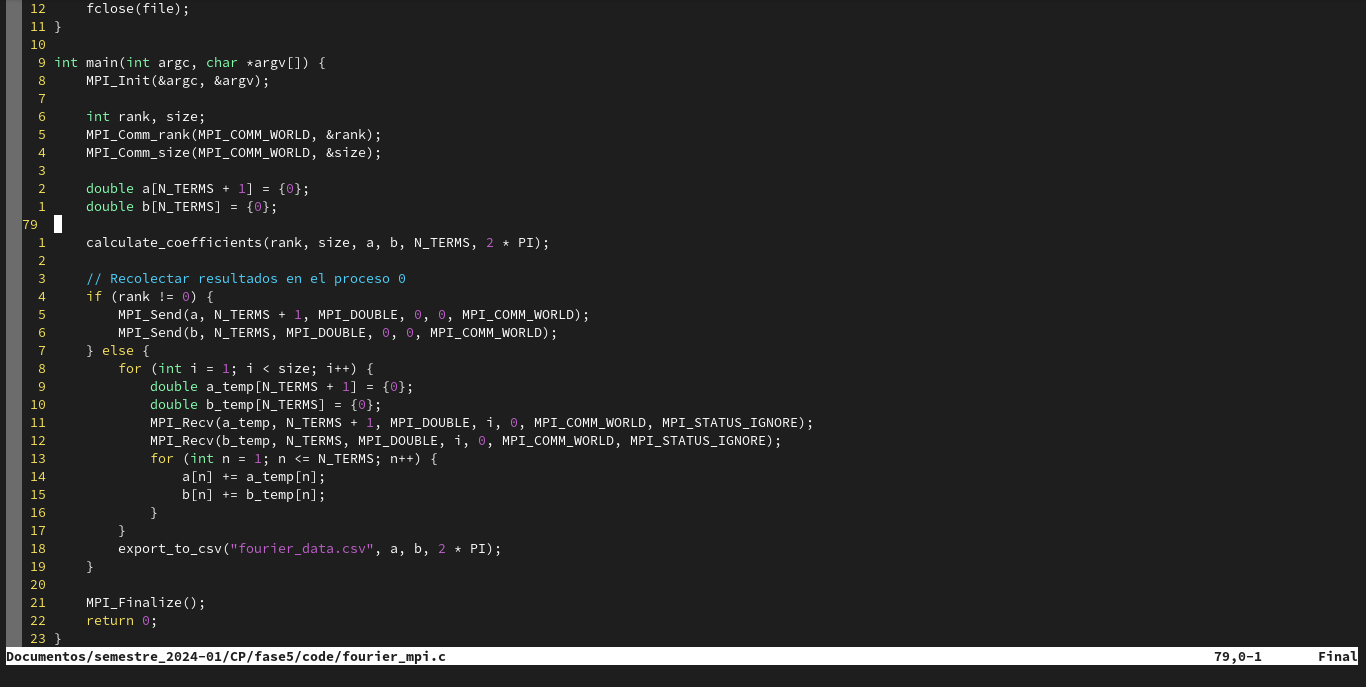
\includegraphics[width=\textwidth]{media/codigo_cuda_4.png}
	\caption{Fragmento del código fuente en C para CUDA. Imagen 4 de 4.}
	\label{img:codigo_cuda_4}
\end{figure}

Este código en C utiliza CUDA para calcular los coeficientes de la serie de Fourier de una función definida, y luego exporta los datos de la función original y su aproximación de Fourier a un archivo CSV.

El programa define algunas constantes, incluyendo el valor de \(\pi\) (\texttt{PI}), el número de términos de la serie de Fourier (\texttt{N\_TERMS}), y el número de puntos en la discretización de la integral (\texttt{N}). La función \texttt{f} es una función definida como \(f(x) = x^4 - 5x^2 - 2x + 1\).

Para calcular los coeficientes de la serie de Fourier, se define un kernel de CUDA (\texttt{calculate\_coefficients\_kernel}) que toma como parámetros los arreglos de coeficientes \texttt{a} y \texttt{b}, el número de términos \texttt{n\_terms}, la longitud del intervalo \texttt{L}, y el paso \texttt{h}. Este kernel se ejecuta en la GPU y realiza la integración numérica para calcular los coeficientes de Fourier \(a_n\) y \(b_n\) utilizando las funciones trigonométricas \(\cos\) y \(\sin\).

La función \texttt{calculate\_coefficients} se encarga de gestionar la memoria en el dispositivo y en el host, y de lanzar el kernel de CUDA. Primero, calcula el coeficiente \(a_0\) en el host y luego lanza el kernel para calcular los demás coeficientes en la GPU. Los coeficientes calculados se copian de vuelta al host una vez que el kernel ha terminado su ejecución.

La función \texttt{fourier\_approximation} calcula la aproximación de Fourier en un punto dado \(x\) utilizando los coeficientes \texttt{a} y \texttt{b}, sumando los términos correspondientes de la serie de Fourier.

Finalmente, la función \texttt{export\_to\_csv} escribe los datos de la función original y su aproximación de Fourier a un archivo CSV. Recorre un rango de valores de \(x\), calcula \(f(x)\) y la aproximación de Fourier en cada punto, y escribe estos valores en el archivo CSV con el formato adecuado.

El \texttt{main} del programa inicializa los arreglos de coeficientes, llama a \texttt{calculate\_coefficients} para calcular los coeficientes de Fourier, y luego llama a \texttt{export\_to\_csv} para exportar los datos a un archivo CSV llamado \texttt{fourier\_data.csv}.
